 \section{Parser Combitators for Path Querying}

Parser combinators provide a way to specify a language syntax in terms of functions and operations on them. 
A parser in this framework is usually a function which consumes a prefix of an input and returns either a parsing result or an error, if the input is erroneous. 
Parsers can be composed by using a set of parser combinators to form more complex parsers. 
A parser combinators library provides with a set of basic combinators (such as sequential application or choice), and there can also be user-defined combinators. 
Most parser combinators libraries, including the Meerkat library, can only process the linear input --- strings or some kind of streams. 
We extend the Meerkat library to work on the graph input.

Meerkat library is a general parser combinators library; by using memoization, continuation passing style and the ideas of Johnson~\cite{Johnson} it supports arbitrary context free specifications. 
This library is closely related to the Generalized LL algorithm and since GLL can be generalized for context free path querying~\cite{GrigorevR16}, the adaptation of Meerkat is reasonable too [!!! переформулировать !!!]. 
It can be done by using an odservation which for (string or graph) parsing we need only to provide function for getting symbols follower by specified position.

The combinators our library provides are presented in table~\ref{table:combinators}. 
Basic parser combinators for mathching strings are implicitly generated whenever a string is used within a query. 
The same generation query can be writen using the library as presented in Fig.~\ref{fig:query1Meerkat}.

\begin{table}[h]
\centering
\begin{tabular}{c|l}
\multicolumn{1}{c|}{Combinator} & \multicolumn{1}{|c}{Description} \\ \hline
{\lstinline!a ~ b!} & sequentional parsing: {\lstinline!a!} then {\lstinline!b!}   \\
{\lstinline!a | b!} & choice: {\lstinline!a!} or {\lstinline!b!}         \\
{\lstinline!a.?!}   & optional parsing: {\lstinline!a!} or nothing   \\
{\lstinline!a.*!}   & repetition of zero or more {\lstinline!a!} \\
{\lstinline!a.+!}   & repetition of at least one {\lstinline!a!} \\
\end{tabular}
\caption{Meerkat combinators}
\label{table:combinators}
\end{table}


\begin{figure}[h]
\begin{lstlisting}
val S: Nonterminal = syn(
   "subclassof-1" ~ S.? ~ "subclassof" |
   "type-1" ~ S.? ~ "type")
\end{lstlisting}
\caption{The same generation query in Meerkat}
\label{fig:query1Meerkat}
\end{figure}


The most exciting feature of our library is that queries can be used as first class values, which means greater generalization and comosition. 
Function \lstinline{sameGen} presented in Fig~\ref{fig:gen} is a generalization of the same generation query which is independent from the environment such as the input graph structure or other parsers.
It can be used for creation of different queries, including the one presented in Fig~\ref{fig:query1Meerkat}: it is the result of application of \lstinline{sameGen} to the appropriate relations (which may be treated  as ``brackets'').
Another application of the \lstinline{sameGen} can be founded in Fig.~\ref{fig:query2Gen}.

\begin{figure}[h]
\begin{lstlisting}
val query1 = syn(sameGen(List(
    ("subclassof-1", "subclassof"),
    ("type-1", "type"))))
\end{lstlisting}
\caption{Query~\ref{query1Meerkat} as an application of \lstinline{sameGen}}
\label{fig:query1Gen}
\end{figure}

\begin{figure}[h]
\begin{lstlisting}
def sameGen(brs) =
  bs.map { case (lbr, rbr) => 
             lbr ~ syn(sameGen(bs).?) ~ rbr } 
  match {
    case x :: Nil => syn(x)
    case x :: y :: xs => 
      syn(xs.foldLeft(x | y)(_ | _))
  }
\end{lstlisting}
\caption{Generic function for same generations query}
\label{fig:gen}
\end{figure}

Running a query over an input graph retrieves the list of pairs $(i, j)$ where each pair corresponds to the set of paths from the node $i$ to the node $j$. 
Running the same generation query from Fig.~\ref{fig:query2Gen} over the graph in Fig.~\ref{fig:graph} returns  $\{(1,0), (1,2)\}$ as a result. 
Internally in Meerkat this paths represented as SPPF~\cite{SPPF}. 
Simplified version of SPPF for this query preseted on Fig.~\ref{fig:sppf} where rounded rectangles represents nonterminals, others rectangles represent productions. 
Every rectangle contains  nontermonal name or production rule, start and end nodes of thr input graph. 
Gray rectangels are start nonterminals.

\begin{figure}[h]
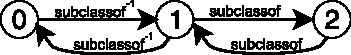
\includegraphics[width=0.45\textwidth]{graph}
\caption{Example input graph.}
\label{fig:graph}
\end{figure}

\begin{figure}[h]
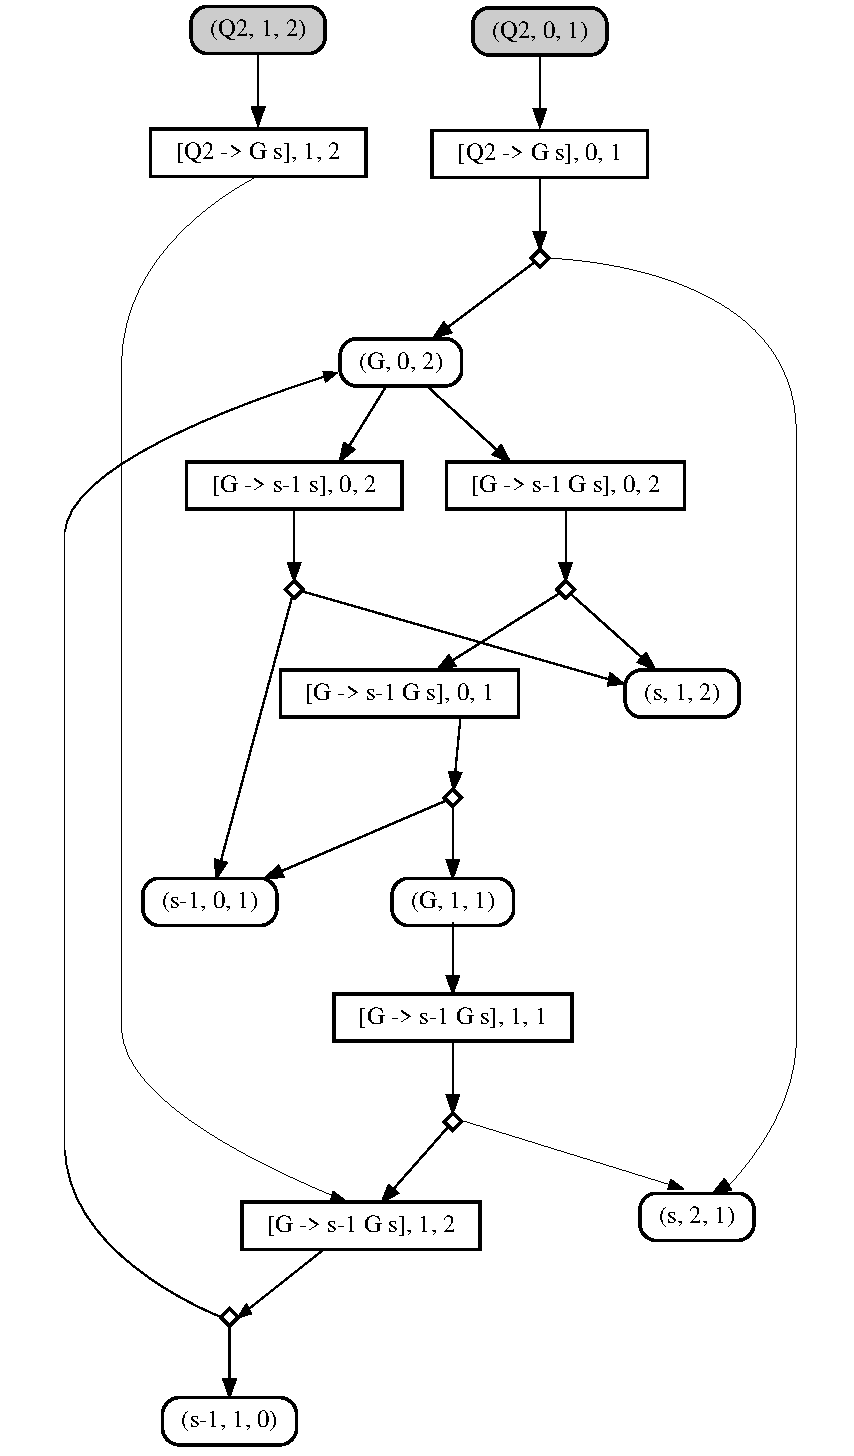
\includegraphics[scale=0.5]{sppf}
\caption{SPPF: result of application the same generation query~\ref{fig:query2Gen} to the graph~\ref{fig:graph}}
\label{fig:sppf}
\end{figure}
